%
%  one figure??
%
%%%%%%%%%%%%%%%%%%%%%%%%%%%%%%%%%%%%%%%%%%%%%%
% Annals of Statistics - Template file
%%%%%%%%%%%%%%%%%%%%%%%%%%%%%%%%%%%%%%%%%%%%%%
\documentstyle[graphicx,leqno,twoside]{aos}
% graphicx added by Joe Felsenstein
%%%%%%%%%%%%%%%%%%%%%%%%%%%%%%%%
\setcounter{page}{1} % <-- To fill at IMS or the typesetter
%%%%%%%%%%%%%%%%%%%%%%%%%%%%%%%%
%%%%%%%%%%%% Definitions %%%%%%%%%%%%%%%%%%
%\def\theequation{\arabic{equation}} % If you don't want the equations counter
                                     % to be reset with each section, 
                                     % outcomment this definition
%%%%%%%%%%%%%%%%%%%%%%%%%%%%%%%%%%%%%%%%%%%

\def\Cov{\mathop{\rm Cov}\nolimits}%       % A sample of proper declaration of
\def\Argmax{\mathop{\rm Arg\,Max}\limits}% a math operator.
\def\Var{\mathop{\rm Var}\nolimits}%
%%%%%%%%%%%% Theorems %%%%%%%%%%%%%%%%%%%%%
% The AOS style allows for theorem-like environments to be numbered throughout
% the paper or to start from one each section (carrying in that case both the
% section number and "theorem" number). If you prefer the first method, declare
% all the environments you need as:
%   \newcounter{<counter_name>}
%   \newtheorem{<counter_name>}{<printed_name>},
% for example, 
%   \newcounter{prop}
%   \newtheorem{prop}{Proposition}
% and that will appear as: 
% 
% Proposition 2. ...
%
% If you want to reset the counter with each new section, use the following
% code: 
%  \newcounter{<counter_name>}
%  \newtheorem{<counter_name>}{<printed_name>}[section],
% for example, 
%   \newcounter{prob}
%   \newtheorem{prob}{Problem}[section]
% and that will appear as: 
% 
% Problem 3.1. ...
%
% We list just some basic counters and leave for the user to decide which
% counters will be used, and should the above mentioned hints about
% declaring the theorem-like environments be used in one or the other way.
\newtheorem{theorem}{Theorem}
\newtheorem{lemma}{Lemma}
\newtheorem{definition}{Definition}
\newtheorem{corollary}{Corollary}
\newtheorem{proposition}{Proposition}
% With proof it is slightly different, and the proof environment does
% expect an argument showing the exact text that will start the proof,
% since this considerably varies from case to case. For example
%  \proof{Proof of the Modified Cramer-Rao Thoerem.}...
%  \endproof,
% where <Proof of the Modified Cramer-Rao Thoerem.> is the actual text to
% start the proof.
% The \proof command can be used also with other similar environments set
% in roman type (not italic as theorems, lemmas, etc.) as Remark, where
% also a halmos (open box) at the end is required:
%   \proof{Remark.}...\endproof
%%%%%%%%%%%%%%%%%%%%%%%%%%%%%%%%%%%%%%%%%%%%%%
% For References AOS provides two possible styles. The standard one
% numbers the references setting the numbers in square brackets. The
% other style that uses only the authors names can be declared by the
% command \NONUMBIB: If you want to use that style, outcomment the
% following line:
%\NONUMBIB
%%%%%%%%%%%%%%%%
\renewcommand{\baselinestretch}{1.0}
\begin{document}
%%%%%%%%%%%%%%%%

%If you have no footnotes, please remove the 1 and 2 below.
\SPECFNSYMBOL{}{1}{2}{}{}{}{}{}{}%

%The following command will set the correct font.

\AOSMAKETITLE

%The following will be filled in later.
%\AOSyr{199X}
%\AOSvol{00}
%\AOSno{00}
%\AOSpp{000--000}
%\AOSReceived{Received XXXX; revised XXXX.}

%Please complete the following information.

\AOSAMS{Primary    ; secondary }
\AOSKeywords{Coalescent; Molecular evolution; genetics}
\AOStitle{Likelihoods on coalescents: a Monte Carlo sampling approach to inferring parameters from population samples of molecular data
\footnote{Supported by NIH grant no. R01 GM-51929 and NSF grant no. BIR-9527687}
}
\AOSauthor{Joseph Felsenstein, Mary K. Kuhner, Jon Yamato, and Peter Beerli}
\AOSaffil{Department of Genetics, University of Washington, Box, 7360, Seattle WA 98195-7360}
\AOSlrh{J. Felsenstein, M. K. Kuhner, J. Yamato, and P. Beerli}
\AOSrrh{Likelihoods on coalescents}
\AOSAbstract{
When population samples of molecular data, such as sequences, are
taken, the members of the sample are related by a gene tree whose
shape is affected by the population processes, such as genetic
drift, change of population size, and migration.  Genetic parameters
such as recombination also affect that genealogy.  Likelihood inference
of these parameters involves summing over all possible genealogies.
There is a vast number of these, so that exact computation is not
possible.  Griffiths and Tavar\'e have proposed computing these likelihoods
by Monte Carlo integration.  Our group is doing this by the
Metropolis-Hastings method of Markov Chain Monte Carlo integration.
We now have, in our {\tt LAMARC} package, programs to do this for constant-sized
and growing populations, and for geographically structured populations.
The bias of the estimator of population growth rate is discussed.
One can also allow for samples stratified in time, as with fossil DNA
or sequential samples from the population of a virus in a patient.
A program for recombining sequences is in progress, and we hope to
put together an object-oriented environment which can cope with
a variety of evolutionary forces.}

%%%%%%%%%%
% Standard LATEX command \maketitle will call the AOS style and set the
% top of the first page of the article in the proper style (but not in
% the proper font).
\maketitle
%%%%%%%%%%

\BACKTONORMALFOOTNOTE{3}

%%%%%%%%%%%%%%%%%%%%%%%%%%%%%%%%%%%%%%%%%%%%%%
\section{Introduction.}

Samples of genes from natural populations of organisms are related by
a genealogy, which is usually unknown.  At the level of the copies of the
genes, such a genealogy would specify where each copy of the gene came from.
Thus, a particular copy that we sample may have come from the mother
of that individual, from her father, from his father, from his mother, and
so on, back in time.  Other copies are doing the same.  As we go back,
occasionally two of these lineages will coalesce, as it happens that
two copies of a gene are descended from the same parental copy.  Thus,
my great-great-great-grandmother might happen to be the sibling of your
great-great-great-grandfather, and the genes we possess might then turn out to
be copied from the same copy in one of their parents.  Such coalescences
are inevitable in natural populations.

Figure 1 shows such a pattern of
ancestry.  Each circle is an individual who has two copies of the gene; we are
concerned not just with the genealogy of the individuals, but with the
genealogy at the gene level.
\begin{figure} % 1.1
\centerline{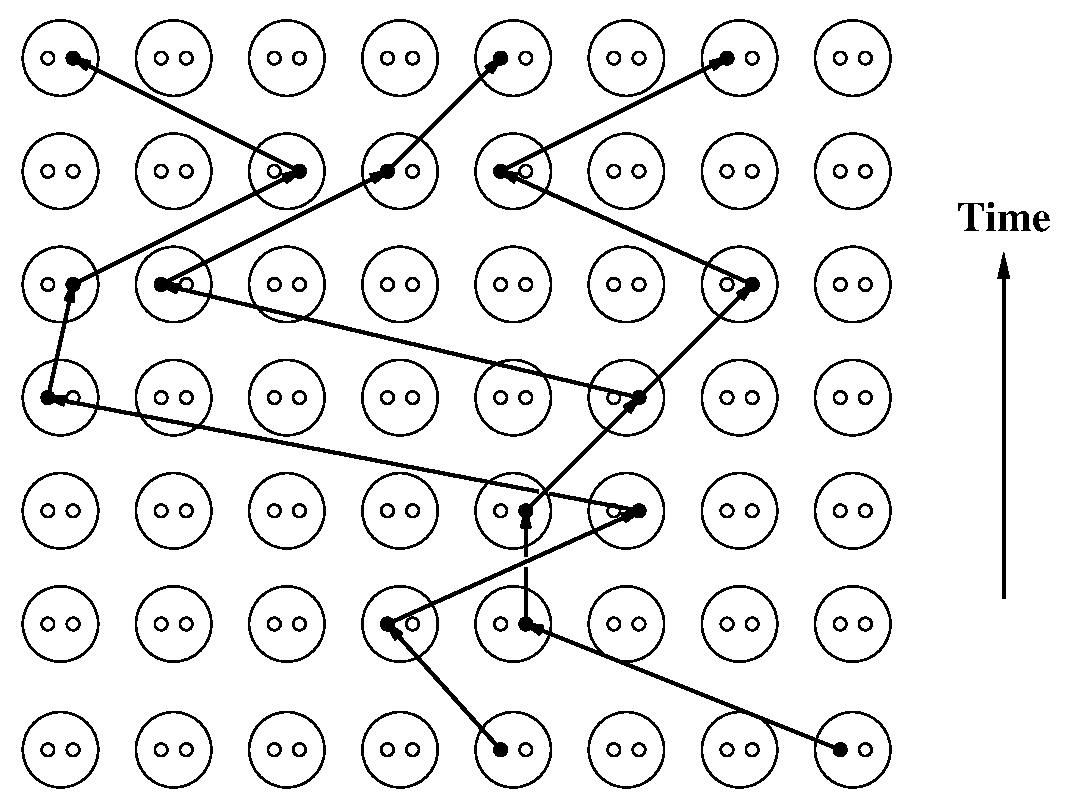
\includegraphics[width=4.5in]{fig1.ps}}
\caption{A coalescent tree of gene copies that is formed in a diagram showing from
which gene in the previous generation each gene copy comes. Large circles are
individuals, small circles are copies of genes.  Three copies in the current
generation trace back to two copies 6 generations earlier.
}
\end{figure}
In the figure, time flows upwards.  The sample consists of three copies of
the gene taken from the latest generation (at the top).  Arrows show the
copies of the gene transmitted from parent to offspring.  When we go backwards
in time along the arrows, we go downwards, and the lineages gradually
coalesce.  The rate of this coalescence is higher in small populations than
in large ones, simply because the chance that the ancestors of two copies of
the gene are the same is greater in a small population.

We have reasonably straightforward models of change in the DNA sequences
of such genes, based on the neutral mutation theory of evolution.  We can,
for example, assume that all sites in the gene change at the same rate $\mu$
per generation,
according to one of the standard Markov models for base subtitution, which
specify probabilities of change among the four states A, C, G, and T.  If
we were to know the genealogy of the copies in detail, statistical estimation
of the rates of mutation would be possible, as well as testing of
hypotheses about the mutational process.  The genealogy is itself the
result of a stochastic process, dependent on $N_e$, the effective population
size.  This would be the population size if the population reproduced
according to an idealized Wright-Fisher model; as it is, it corrects for
some departures from such a model.  We could imagine using the genealogy
to estimate $N_e$ and test hypotheses about it.

However, we don't know the genealogy.  We must therefore integrate over our
uncertainty about it.  This turns out to confound $N_e$ and $\mu$, and
create a large computational problem.  In this paper, we will outline
the problem, our own Markov Chain Monte Carlo approach, and relate it to the
work of Griffiths and Tavar\'e, who have suggested another Monte Carlo
sampling approach.  We will also sketch how population growth, migration,
recombination, and fossil DNA sequences can be accomodated in our scheme.

\section{The Coalescent.}

It has been known since the work of Sewall Wright, in the 1930's, that
if we choose two copies of a gene from a random-mating population, the
time since their common ancestor is geometrically distributed, with expectation
$2N$ generations. (For the moment we use $N$, the actual population size, as
we are dealing with idealized models).  As $2N$ is typically reasonably large, it is also
well-approximated by an exponential distribution with that expectation.
In 1982 Kingman \cite{Kingman82a, Kingman82b, Kingman82c} generalized this to $n$ copies by defining the
coalescent process, and proving that the distribution of the genealogies
of the $n$ copies converges to it when scaled properly.  While Kingman's
methods were sophisticated, the resulting distribution is easy to
describe and use.  This is fortunate, for Kingman's result is fundamental to
the analysis of population samples of DNA sequences.

In the coalescent in a population whose size is $N$, one can
sample from the distribution of the possible genealogies of $n$ copies by
the following procedure:
\begin{enumerate}
\item Set $k = n$ and $T = 0$.
\item Draw a random quantity $u_k$ from an exponential distribution with
expectation $4N/(k(k-1))$.
\item Pick two of the $k$ copies of the gene at random, without replacement.
\item Create a node of the genealogical tree which is the immediate common
ancestor of these two copies, and which existed $T + u_k$ generations
before the present.
\item Set $T = T + u_k$.
\item Replace these two copies by this common ancestor and set $k = k - 1$.
\item If $k = 1$ we are done.  Otherwise return to step 2.
\end{enumerate}

Thus we go back through a series of exponential time intervals, combining
randomly chosen pairs of lineages, until we get a complete tree.  The
expected time to reach the common ancestor of all copies is $4N(1-1/n)$
generations.  The lineages combine rapidly at first, then more slowly as we
go back, and the last two are expected to take $2N$ generations to find their
common ancestor, more than half of the expected time.  An interesting
implication of
the coalescent is that a sample of modest size has an excellent chance that
its common ancestor will also be the common ancestor of all copies of the
gene in the population.

Kingman's coalescent is an approximation, valid when $n^2 \ll N$, but it is
in practice extraordinarily accurate.  Given the departures that real
populations show from any of these idealized models, inaccuracy of
Kingman's approximation is the least of our worries.  Kingman's coalescent
defines the prior distribution of genealogies, and has given its name to the
whole area: researchers studying ancestry of samples of genes from populations
are said to be working on coalescents.

There are many possible departures from the idealized Wright-Fisher model
that underlies Kingman's result, but the coalescent is in effect a
diffusion approximation.  Many different models of reproduction of
single populations will have the same diffusion approximation, and hence
the same coalescent process, provided we replace the actual population size
$N$ by the appropriate effective population size $N_e$.

\section{Likelihoods.}

\def\Prob{\mathop{\rm Prob}\nolimits}

The coalescent gives us a prior distribution of the genealogy $G'$, which
has its intervals expressed in generations.  As a product of exponential
densities, it is easily written down and easily computed.  Its density
function is
\begin{equation} % 3.1
f\left(G'|N_e\right) =
\prod_{k=2}^n {2 \over 4N_e}\exp\left(- {k(k-1) \over 4N_e} u_k \right)
\label{eq:basic}
\end{equation}
where $u_k$ is the length of the interval during which the genealogy $G'$
has $k$ lineages.  If we were  able to observe the coalescence intervals $u_k$,
we could estimate $N_e$.  Note that the event that actually occurs brings in
a factor of $2/(4N_e)$ rather than $k(k-1)/(4N_e)$ as we know which two
lineages have coalesced.  The product of these factors of $2/(k(k-1))$
represents the
probability of sampling the particular ``labelled history" \cite{Edwards70}
from among all those possible.

Of course, we do not actually observe coalescence intervals.  For most
kinds of contemporary data, we can observe only the differences between
the members of our sample.  For example, for DNA sequences, we can see
the number of positions (sites) at which the molecules differ.  That
gives us a picture of the coalescence times, but only a clouded picture.
We need to make inferences about parameters such as $N_e$ by using a
model of the change in the DNA.  The notion of a molecular clock
provides such a model.  We assume a Markov process operating independently
at each site in the DNA, with a mutation rate $\mu$.  By equating long-term
change to mutation, we are implicitly basing ourselves on the neutral
mutation model of evolution made famous by Motoo Kimura
\cite{Kimura68,Kimura83}.
We can use a stochastic model of DNA change, and make assumptions of
independence of change in different sites and in different lineages, to compute
the probability of the observed sequences $D$ given a genealogy $G'$.
One of us (J.F.) has outlined how to do this
\cite{Fels81} and Ziheng Yang, Gary Churchill, and he
have more recently shown how to incorporate autocorrelated variation
of evolutionary rates from site to site using a Hidden Markov Model approach
\cite{Yang93, Yang94, Yang95, Fels96}.

We cannot be certain of the genealogy $G'$.  In fact, it is the role of
the data to illuminate it, however dimly.  To compute the likelihood of the
coalescent parameter $N_e$ and the mutation rate $\mu$ given the data $D$,
we must integrate over all possible genealogies \cite{Fels88, Fels92}
\begin{equation} % 3.2
\Prob\left(D|N_e, \mu\right) = \int_{G'} f(G'|N_e) \Prob(D|G', \mu).
\label{eq:intG}
\end{equation}
We describe the integration below.
The probability of $D$ given $G'$ and $\mu$ which appears on the right is the
probability calculated by our Markov process model of evolution, the same
quantity that is computed in maximum likelihood inference of phylogenies.
The quantity $\mu$ is a rate of mutation per generation; in more complex
cases this may be replaced by several parameters.

Neither of the terms inside the integral in equation \ref{eq:intG} is hard to compute.
The quantity $f$ is given by (3.1) and the other probability requires
effort proportional to the total number of DNA bases in our sample, times
the square of the number of states at a site, which is 4.  The computational
problem comes from the vast size of the space of genealogies $G'$.  The space
of values of $G'$ is a union of a very large number of Euclidean spaces.
Edwards \cite{Edwards70} enumerated these: they are his ``labelled histories".
With $n$ sequences there are $n!(n-1)!/2^{n-1}$ of them, so that with only
10 sequences there are $2.571\times 10^9$ labelled histories.  Each
one of these has $n-1$ node times.  The integration in (3.2) must be over
all values of these, so that each of these billions of terms integrates over
$n-1$ dimensions.  Clearly there is a computational problem here.

All attempts to find mathematical simplifications for this integration
have so far failed.  Nevertheless two groups -- Griffiths and Tavar\'e and
ourselves -- have attempted to use Monte Carlo integration.  This can work
because many of the billions of possible labelled histories make rather
little contribution to the integral, because they lead to very low values of the
term $\Prob(D|G')$.  We will describe our approach first, and then show the
relationship between the two approaches, which appear at first sight to be
quite different.

\section{A Metropolis-Hastings approach.}

Our approach has been to use Markov Chain Monte Carlo sampling, in particular
the Metropolis-Hastings method \cite{Metropolis53, Hastings70}.  We want to sample from
the terms of (3.2) using importance sampling, with our importance
function being as close as possible to the
the that is being integrated.  Our approach
for the simplest case -- a single population of constant size,
with no recombination -- is outlined by Kuhner et. al. \cite{Kuhner95,
Kuhner97}.

In that case, it turns out that we can change the time scale of the
genealogies.  The entities $G'$ have their node times given in generations.
Instead we can rescale them to be in units of $1/\mu$ generations, where
$\mu$ is the underlying neutral mutation rate of the DNA model that we
use.  Thus if a node in the genealogical tree is 100,000 generations
ago, and the underlying mutation rate $\mu$ is $10^{-7}$, when rescaled
the node is 0.01 mutations ago.  These are of course expected mutations
per site, not actual mutations.  Informally, we can write this by
saying that the genealogy is now $G$ rather than $G'$, and
\begin{equation} % 4.1
G = \mu G'.
\end{equation}
The result of this change of variables is of course to alter the
density $f$ as well.  The coalescence intervals $u_k$ in (3.1) are
replaced by $v_k = \mu u_k$, and a factor of $1/\mu$ comes into each
term in the resulting density as well.  The result is the density:
\begin{equation} % 4.4
g(G|\Theta) = \prod_{k=2}^{n} {2 \over \Theta}\exp\left(- {k(k-1) \over \Theta} v_k \right)
\end{equation}
where $\Theta = 4N_e \mu$.  This resembles closely the widely-used parameter
$\theta$ that is frequently estimated in evolutionary genetics, except that
it contains the neutral mutation rate per site rather than per locus.

The result of this change of scale is that the probability $\Prob(D|G', \mu)$
can be replaced by $\Prob(D|G)$, as the branch lengths of $G$ are already
multiplied by the mutation rate.  In most DNA models, the elapsed time $t$
in generations must be multiplied by a rate of mutation $\mu$ before it can be
used.  If we are given the product $\mu t$ we can compute the transition
probability directly from it.  The result is that (3.2) now becomes:
\begin{equation} % 4.5
\Prob\left(D|\Theta\right) = \int_G g(G|\Theta) \Prob(D|G).
\end{equation}
If there were more parameters than $\mu$, one would have to change
$\Prob(D|G)$ by adding ratios of parameters, such as $\Prob(D|G, \mu_2/\mu_1)$.
Our objective becomes computing the likelihood of the parameter $\Theta$.

To approximate the integral we take as our importance function the
quantity $g(G|\Theta) \Prob(D|G)$, which immediately raises the issue of
what value of $\Theta$ to use.  Ideally one would want to sample at
the maximum likelihood value of $\Theta$, but we cannot know in advance
what this will be.  Our strategy has been to make a rough estimate of $\Theta$,
which we call $\Theta_0$, and use that for an initial sampling,
sampling from $g\left(G|\Theta_0\right)\Prob(D|G)$.  We sample genealogies
$G_1$, $G_2$, $\ldots$, $G_m$ by taking an initial genealogy and making
successive alterations to it, doing acceptance/rejection sampling appropriately
according to a Metropolis-Hastings algorithm.  This forms a Markov chain of
genealogies.  We use that for an initial sampling, then find a
maximum likelihood value based on the sample from that first Markov chain.
This is then taken as the provisional value for
a second Markov chain, and so on.  We have usually run 10 of these chains,
then two much longer ones at the end.  The final likelihood curve is computed
from the second of these long chains.  In our programs the user can customize
the number and lengths of the chains.

\section{Importance sampling and likelihood curves.}

One useful property of Metropolis-Hastings sampling is that we can
estimate the whole likelihood curve from a single run of a Markov chain,
rather than having to compute each point on the likelihood surface from a
separate run.  Suppose that we sample $m$ genealogies from a Markov chain
which has its equilibrium distributiion proportional to
$g(G|\Theta_0) \Prob(D|G)$.  Call
the sampled genealogies the $G_i$.  The usual importance sampling formula
for Monte Carlo integration gives:
\begin{equation} % 5.1
{~~~~}\,\,\,\int_G g(G|\Theta) \Prob(D|G) \simeq \frac{1}{m} \sum\limits_{i=1}^m {g(G_i|\Theta) \Prob(D|G_i) \over  g(G_i|\Theta_0) \Prob(D|G_i)} = \frac{1}{m}\sum\limits_{i=1}^m {g(G_i|\Theta) \over  g(G_i|\Theta_0)} 
\end{equation}
this allows us to estimate the likelihood for other values of $\Theta$ from
a run of the Markov chain at $\Theta_0$.  Note that the likelihood curve
depends only on the Kingman priors of the sampled $G_i$ at $\Theta$ and
at $\Theta_0$.  This makes it seem that the data are not involved at all; they
actually affect the Markov Chain Monte Carlo sampling process and affect the
final likelihood through their effect on which $G_i$ are sampled.

\section{The Markov Chain sampling.}

Our samples of the genealogies $G$ must come from a distribution
proportional to $g(G|\Theta_0) \Prob(D|G)$.  We achieve this through
a sampling based on conditional coalescents.  A conditional coalescent may
be described as a distribution on $G$ that has its density proportional to
the coalescent density $g(G|\Theta_0)$ on some domain of $G$'s, and has
density 0 elsewhere.  In our programs the conditional coalescents are
created by a process of dissolving part of a tree, and reforming that part
by allowing lineages to sample their ancestry randomly according to a
conditional coalescent.  In the original paper by Kuhner et. al. \cite{Kuhner95},
the region of the tree that was dissolved had a single lineage at its
base and three lineages at its top.  The three lineages, which were not
necessarily contemporaneous, were then re-formed into a tree by allowing
them to coalesce, but requiring that all three coalesce into a single
lineage by the time the base of the dissolved region was reached.  The
details of how this was done will be found in that paper.

More recently, we have changed to a different conditional coalescent
suggested by Peter Beerli.  In this, a lineage is selected, and is
disconnected from the genealogy, with the lineage being dissolved back up
the tree to the next highest coalescent node.  It is then allowed to
sample its ancestry downwards (backwards in time) until it re-connects
to the tree.  Note that sometimes this will mean it reconnects below the
previous root of the tree.  Figure 2 shows this process in a  single
population.
\begin{figure} % fig. 2
\centerline{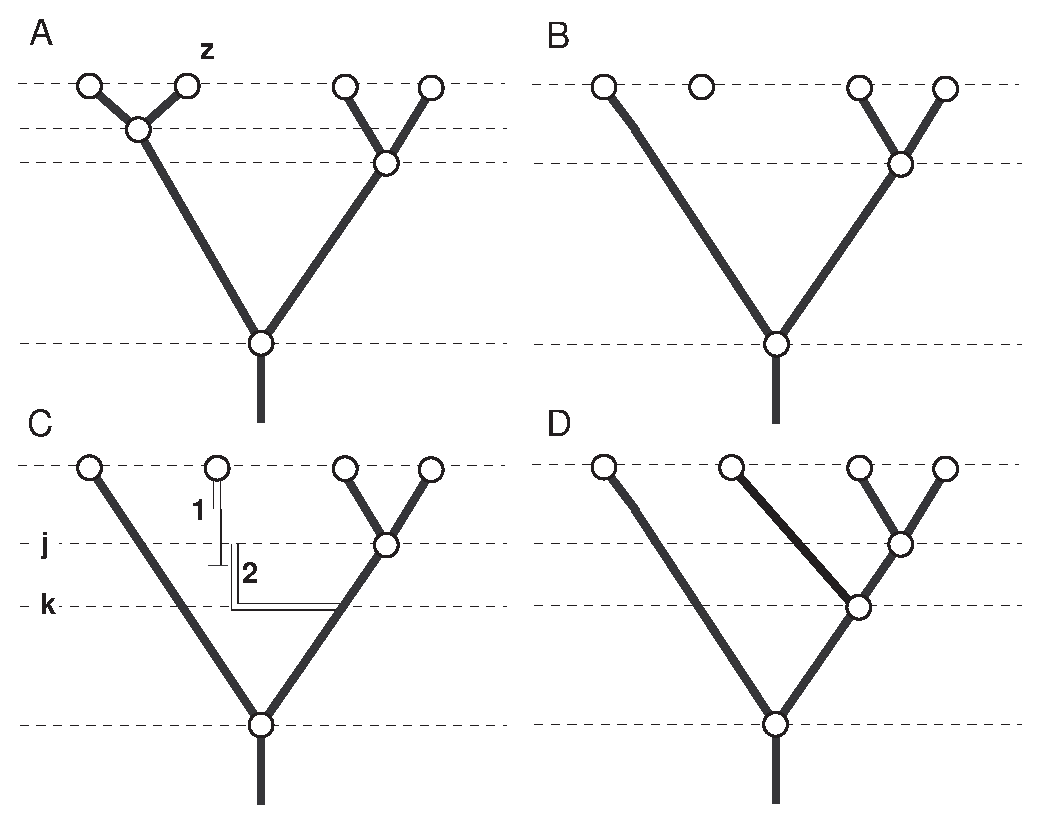
\includegraphics[width=4.5in]{fig2.ps}}
\caption{A conditional coalescent method of altering a tree.  A
single lineage is chosen at random to be altered (the lineage below z in
A).  It is removed from the tree (B) and then its coalescence with the
remaining lineages is simulated (C).  Tree D shows the result.
}
\end{figure}
A branch of the tree is chosen at random.  In this case it is the one below
tip $z$ (tree A).  Tree B shows the tree with that branch removed.  In
tree C we see the process of simulating the conditional coalescence of that
lineage with the remaining ones.  During the topmost interval of the tree
(the time down to line $j$), the instantaneous rate of coalescence of that
lineage with each of the three others is $2/\Theta_0$, for a total of
$6/\Theta_0$.  We generate an exponential random variate with mean $\Theta_0/6$,
which is the time until coalescence of that lineage with one of the three
others.  In this case (line 1 in tree C) the time is too long, and takes
the lineage past line $j$.  We then consider the lineage to have remained
distinct back as far as line $j$.  Starting at that time, we have two
other lineages, for a total instantaneous rate of coalescence of $4/\Theta_0$.
We then draw an exponential variate with mean $\Theta_0/4$.  This time, which
defines line $k$, turns out to be a time above the next coalescence, which
is the root of the tree.  So we connect our new lineage to the tree at the
time of line $k$, choosing one of the two lineages as the one to which it
will be connected.  The resulting tree is D.

Note that it is possible for any of the lineages, other than the one that
is below the root, to be chosen to be dissolved, and it may reconnect to the
tree below the original root.  The method requires one exponential variate
to be generated
for each coalescence interval on the remaining part of the tree.  If there
are $m$ other lineages in an interval, the instantaneous rate of coalescence
with them is $2m/\Theta$.

Having proposed this change, we decide whether to accept it.  The method of
generating the new tree is a conditional coalescent, which means that if the
old tree is $G_{old}$ and the new tree $G_{new}$, then 
\begin{equation}
\Prob\left(G_{new}|G_{old}\right) = K Prob\left(G_{new}|\Theta_0\right)
\end{equation}
for some constant $K$, as the density from which $G_{new}$ is drawn is
proportional to the coalescent density.  An analogous equation holds for
$\Prob\left(G_{old}|G_{new}\right)$.  In constructing the rule for
acceptance and rejection, we use these in the Hastings ratio terms,
accepting the new tree if a uniform random fraction $r$ satisfies
\begin{equation}
\begin{array}{c c l}
r & < & {\Prob\left(G_{old}|G_{new}\right) \over \Prob\left(G_{new}|G_{old}\right)}
{\Prob\left(G_{new}|\Theta_0\right)\Prob\left(D|G_{new}\right)  \over \Prob\left(G_{old}|\Theta_0\right)\Prob\left(D|G_{old}\right) }\\
  &  & \\
 & < & {Prob\left(G_{old}|\Theta_0\right) \over Prob\left(G_{new}|\Theta_0\right) }
{\Prob\left(G_{new}|\Theta_0\right)\Prob\left(D|G_{new}\right) \over \Prob\left(G_{old}|\Theta_0\right)\Prob\left(D|G_{old}\right) }\\
  &  & \\
 & < & {\Prob\left(D|G_{new}\right) \over \Prob\left(D|G_{old}\right) }.
\end{array}
\end{equation}

Thus the conditional coalescent causes cancellation of the Hastings terms and
the Kingman prior term, leaving only the ratio of the likelihoods of the trees.
These would be the likelihoods of these genealogies, given the data, if the
genealogies were treated as parameters (which they are not).  The machinery
to compute likelihoods on genealogies is the same as it is on phylogenies, and
it is well-enough known (e.g. \cite{Fels81}) not to need to be treated here.
Note that we can use any type of data for which such likelihoods are available, 
including DNA sequences, microsatellite copy numbers, restriction sites, and
even isozyme mobilities.  Note also that we have only modified part of the
tree, so that we need only recalculate the likelihoods for the
parts of the two trees that differ, a considerable saving.
The rearrangement strategy described here has some similarity to that used
by Li et. al. \cite{Shuying} but their strategy dissolves only branches leading
to tips, and does not use the conditional coalescent for reattachment.

As an example, Figure 3 shows the likelihood curve generated by a run of
on the mitochondrial DNA data set of Ward et. al. \cite{Ward91}.  The estimate of $\Theta$
is 0.0396.  Taking an interval two units of log-likelihood below the maximum
suggests that the estimate lies between about 0.03 and 0.055.
\begin{figure} % 3
\centerline{\includegraphics[width=3in]{fig3.ps}}
\caption{The log-likelihood curve for $\Theta$ for the data of Ward et. al.}
\end{figure}
This curve was generated by two long chains of 12,000 steps each, sampling
trees every 20 steps.  Further details are given by Kuhner et. al. \cite{Kuhner95}.

The method is computationally feasible on workstations or fast desktop
computers.  Computational effort seems to rise slowly with the number of
sequences, especially since we can re-use many of the likelihood computations
from one tree to the next.  If only part of a tree has changed we can
re-use the likelihoods from the rest of the tree.  However there are no
easy generalizations about how long the Markov chains must be run.

\section{The method of Griffiths and Tavar\'e.}

Our Monte Carlo sampling approach was preceded by the pioneering and
innovative method of
Griffiths and Tavar\'e \cite{GT94a, GT94b, GT94c}.  At first sight their method appears to
bear no relation to ours, and to have considerable advantages over it.
A close examination shows that the two methods are related, and makes
clear the advantages and disadvantages of our approach.

Griffiths and Tavar\'e have as their objective the same likelihood function
that we compute.  They form a system of recurrence equations expressing this
likelihood in terms of likelihoods for data sets that have resulted from
one fewer evolutionary event.  In principle, recursive evaluation of these
equations, as in an earlier paper by Griffiths \cite{Griffiths89}, will yield the desired
likelihood.  However, the recursion expands rapidly, and one must therefore
use some approximate method of evaluating it.  Griffiths and Tavar\'e 
\cite{GT94a, GT94b, GT94c} choose
sample paths down through the recursion randomly.  The great advantages of
this method are that the computations are rapid, and each such sample
path is independent of all the others.  By contrast, our samples are
autocorrelated, leading to serious problems knowing how long to continue
the sampling.  In each of our samples, the likelihood of a tree must be
computed.  Even if parts of the computation can be re-used, this is much
more effort than is needed for their method.

Each step in their sampling goes back one level in the recursion, and
amounts to a decision as to what the next most recent event in the
genealogy is.  The sequence of choices that Griffiths and Tavar\'e make
corresponds to a sequence of events in evolution.  Going backwards in time,
their events are mutations and coalescences, plus choices of the
ancestral nucleotides at each site.  Figure 4 shows such a history
of events leading to a set of four DNA sequences.  It corresponds to one
\begin{figure} % 4
\centerline{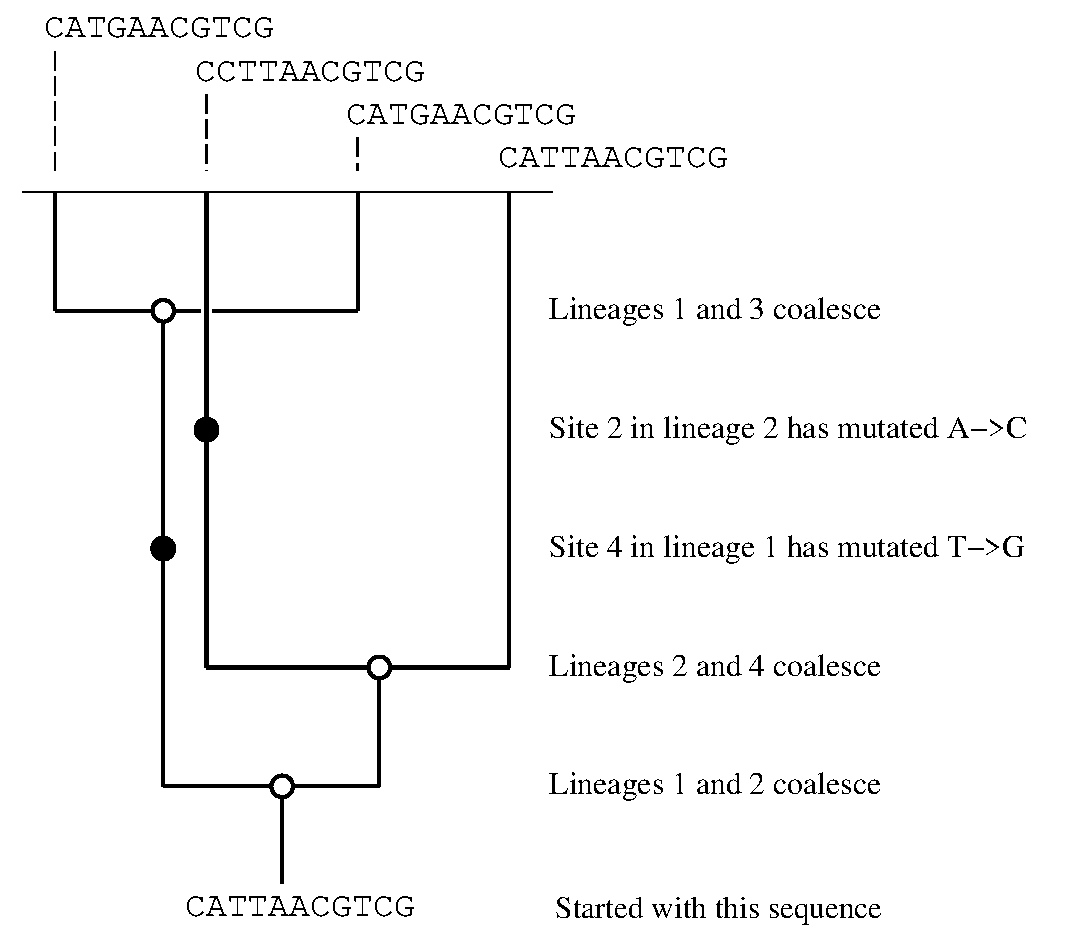
\includegraphics[width=4.5in]{fig4.ps}}
\caption{A history of mutation, coalescences, and ancestral nucleotide choices
that could result in a given set of four sequences. Such histories
are, in effect, what Griffiths and Tavar\'e's method samples.  The
events are described from a point of view looking backwards in time from
the present.}
\end{figure}
path through their recursion.  Note the difference between such a history
($H$) and the genealogy ($G$) that we sample.  Our genealogy has branch
lengths; theirs does not, at least in the simplest case.  They specify
the place of occurrence of each mutation, while our likelihoods must sum
over all possible placements of mutations on the tree.  Nevertheless, we
can regard their method as Monte Carlo integration.  We can make an
equation analogous to our equation \ref{eq:intG}:
\begin{equation} % 7.1
L = \Prob(D|\Theta) = \sum_H \Prob(D|H) \Prob(H|\Theta),
\end{equation}
where $H$ is a history of events, corresponding to a sequence of choices
in Griffiths and Tavar\'e's recursion.  The histories that they sample
have the property that they must always lead to the observed sequences.
Thus $\Prob(D|H)$ is, trivially, always 1.  The term $\Prob(H|\Theta)$ is
simply the product of probabilities of the individual events in $H$.  In
the history shown in Figure 4, the most recent event could have been a
mutation in any of the 11 sites in any of the four sequences, and each
could have come from any of three other nucleotides.  The particular
event that is shown is a coalescence.  There are only two sequences (1 and 3)
that are identical, and thus could have coalesced at this point.  The
rate of coalescence for this pair will be $1/(2N_e)$.  The next event is
a mutation.  If we use, for simplicity, a symmetric Jukes-Cantor model of
evolution, the rate of occurrence of a particular mutation from {\it C}
to {\it A} at a particular site will be $\mu/3$, where $\mu$ is the
total mutation rate per site.

Consider all possible histories $H$, those that lead to the observed sequences
as well as those that do not.  As the most recent event, there are
$4\times 11\times3$
possible mutations, and $4\times 3/2$ possible coalescences.  The fraction
of this probability contributed by the most recent coalescence in Figure 4 
is then $(1/(2N_e))/\left(6/(2N_e)+44\mu \right)$, which turns out to be
$1/(6 + 22\Theta)$.  Continuing in this fashion we can calculate
the probability $\Prob(H|\Theta)$ of the particular sequence of events in Figure 4 to be
\begin{displaymath}
\left({1 \over 6+22\Theta} \right)\left({\Theta \over 18+99\Theta} \right)\left({\Theta \over 18+99\Theta} \right)\left({2 \over 6+33\Theta} \right)\left({1 \over 1+11\Theta} \right)\left(\frac{1}{4}\right)^{11}.
\end{displaymath}
The last term is the probability that the initial DNA sequence is as shown
in Figure 4.
In effect what Griffiths and Tavar\'e do is to sum over all such histories,
adding up this quantity for all those that lead to the observed data. 

Griffiths and Tavar\'e at each stage are considering all possible most
recent events that could have led to the observed sequences.  They use
importance sampling, by sampling at each stage from among the possible
events in proportion to their rate of occurrence.  Thus at the first
stage in the above calculation, they choose among the one possible coalescence
and the 33 possible mutations in proportion to the contributions each would
make to the numerator (in that case $1/(2N_e)$ versus $\mu/3$).
This needs the usual importance sampling correction.   Their sampling is
done, as ours is too, at a trial value $\Theta_0$.  Suppose that $f$ is the
probability
$\Prob(H|\Theta)$, unconditioned on the data, and $h$ is the
probability for the distribution from which we sample instead.  The
importance sampling correction is
\begin{equation} % 7.9
L(\Theta) = {\cal E}_f\left[\Prob(D|H)\right] = {\cal E}_h\left[{f \over h}\Prob
(D|H)\right]
\end{equation}
and since for $h$ we always have $\Prob(D|H) = 1$, the likelihood is just
the expectation over $h$ of $f/h$.

A history $H$ consists of a series of choices.  Suppose that history $H_i$
has at stage $j$ a series of possibilities, with the terms of the Griffiths/Tavar\'e
recursion being the $a_{ijk}(\Theta_0)$.  Suppose that one that is actually
chosen in history $H_i$ has term $b_{ij}(\Theta_0)$.  Then the probability of
having taken this choice is
\begin{equation} % 7.9
{b_{ij}(\Theta_0) \over \sum_k a_{ijk}(\Theta_0)}
\end{equation}
and the probability of the history is the product of this ratio over all $j$,
the number of these depending on the number of events in history $H_i$.
This is the expression for $h$.  The distribution $f$ is similar except that
it has $\Theta$ in place of $\Theta_0$, and a wider range of possible
events, including those which conflict with the data.  The full set of
events at stage $j$ in this distribution we call the $c_{ijk}(\Theta)$.

We end up with
\begin{equation} % 7.10
L(\Theta) = {\cal E}_h\left[{\left({\Pi_j b_{ij}(\Theta) \over \Pi_j \left(\sum_
k c_{ijk}(\Theta)\right)}\right) \over \left({\Pi_j b_{ij}(\Theta_0) \over \Pi_j
 \left(\sum_k a_{ijk}(\Theta_0) \right)}\right)}\right]
 = {\cal E}_h \left[\Pi_j{b_{ij}(\Theta) \over b_{ij}(\Theta_0)}{\sum_k a_{ijk}(\Theta_0) \over
 \sum_k c_{ijk}(\Theta)}\right]
\end{equation}
Griffiths and Tavar\'e's method consists of sampling from $h$ to approximate
this expectation by averaging the ratio on the right.  A careful reading of
their papers will show that the above expression is precisely what they
compute.  Thus their method too can be considered a Monte Carlo integration
method with an importance function.

Given the independence of their samples, and the rapidity with which they
can compute them, one might expect their method to be unequivocally
superior to ours.  We are, after all, burdened by more computation and
autocorrelated samples.  The difficulty with their method is that the
distribution $h$ from which they sample does not sample from the histories
in proportion to their contribution to the likelihood.  There is thus some
wasted effort.  By contrast our Metropolis-Hastings sampling is supposed
to sample from genealogies in proportion to their contribution to the
likelihood.  We thus have reason to hope that our method might do
better in some cases.  The problem is most easily seen when considering
how Griffiths and Tavar\'e's method will handle two DNA sequences.  If those
sequences happen to differ by (say) 2 bases, the mutational events that are
sampled will include not only the precise changes needed to make the two
sequences identical, but also all other changes in all other sites.  Thus
a great deal of sampling may be needed to sample from the events that
contribute most of the likelihood.   Griffiths and Tavar\'e \cite{GT94c} have
worried aloud about this very issue.
 
\section{Population growth.}

The model of an isolated population of constant size can be extended by
allowing the population to grow exponentially.  Griffiths and Tavar\'e
\cite{GT94a}
have done so, and so have we \cite{Kuhner98}.  Our program {\tt FLUCTUATE} is currently
in distribution.  In a population of effective
size $N_e(t)$ with $k$ lineages, the
rate of coalescence is $k(k-1)/(4N_e(t))$.  If the effective
population size grows
exponentially at rate $r$, then when $t$ is the time back from the present
(``dual time"),
\begin{equation} % 8.1
N_e(t) = e^{-rt} N_e(0)
\end{equation}
Taking this into account in the time to coalescence, that density function
is \cite{Kuhner98}
\begin{equation} % 8.2
f(t) =  e^{\left[-\frac{k(k-1)}{4N_e(0)r}\left(e^{rt}-1\right)\right]} e^{rt} \frac{2}{4N_e(0)}.
\end{equation}
This can be used to make a counterpart to equation \ref{eq:basic} straightforwardly.
Griffiths and Tavar\'e \cite{GT94a} have used this for joint likelihood inference of
the current value of $\Theta$ and the growth rate.  We have more recently
produced a Metropolis-Hastings algorithm \cite{Kuhner98} for a similar model.

Once the mutation rate $\mu$ is introduced and the branch lengths of the
genealogical trees rescaled in units of expected mutations per site,
the parameters of the likelihood turn out to be the current value of
$4N_e(0)\mu$, called $\Theta$, and the growth rate per unit branch length,
which is $g = r/\mu$.  The likelihood surfaces in these parameters usually 
contain long, narrow ridges.  At any
given value of $g$, the estimation of $\Theta$ is reasonably accurate,
but there is usually a long, narrow, slightly curving ridge whose top is
nearly flat.  It runs nearly parallel to the $g$ axis, but curving
gradually upwards as higher values of $g$ are reached.

There turns out to be surprisingly little power to estimate
$g$, except in cases where the true value of $g$ is large.  Even more
surprising is
the strong bias in the estimate of $g$.  When data sets are generated from a
model that has no population growth, they much more often cause us to
estimate a large positive $g$ than a negative $g$.  The behavior is so
startling as to make us wonder whether it simply be the result of a program
bug.  

We can verify that the bias is real by using (8.12), and considering the case
of a sample of size 2 ($n = 2$).  Suppose that we had very long, nonrecombining
sequences.  That would allow us to make a precise estimate of the
rescaled time $T = \mu t$ to coalescence.  The likelihood function can be written
in terms of $g$ and $\Theta = 4N_e(0)\mu$.
\begin{equation} % 8.3
\Prob(T |\Theta, g) =  e^{\left[-\frac{2}{\Theta g}\left(e^{gT}-1\right)\right]} e^{gT} \frac{2}{\Theta}.
\end{equation}
In the case of a sample of size 2, let us assume that $\Theta$ is known, and set
in (8.13) to its true value, and that we are estimating $g$.  There is no
explicit formula solving for the maximum likelihood estimate $\hat{g}$
in terms of $T$, but the likelihood can be maximized numerically.
Now imagine a population whose true growth rate is zero, and whose
value of $\Theta$ is known to be 1.  The scaled coalescent time $T$ for
sample size 2 will be distributed exponentially with mean 0.5.

In Figure 5, the maximum likelihood estimate $\hat{g}$ is shown for
quantiles of that distribution.  It is striking that 87\% of the time
the estimate is positive, and very strongly positive for small
coalescent times (below 0.08 the curve is too high to fit onto this
figure).  The other 13\% of the time the estimate is negative,
though only moderately so.  The bias in $\hat{g}$ can be seen: it is the
average height of the curve, which is strongly positive.  Note that the
growth rate scale means that $g=20$ implies growth of the population
by a factor of $e^{10}$ during the expected time for two samples to
coalesce.  Even at the median of the coalescence times, the bias implies
that we infer growth by a factor of $e^{2.166}$ during the average coalescence
time.  As our Metropolis-Hastings algorithm is not used here, this calculation
is an independent check of the reality of the bias.
\begin{figure} % 5
\centerline{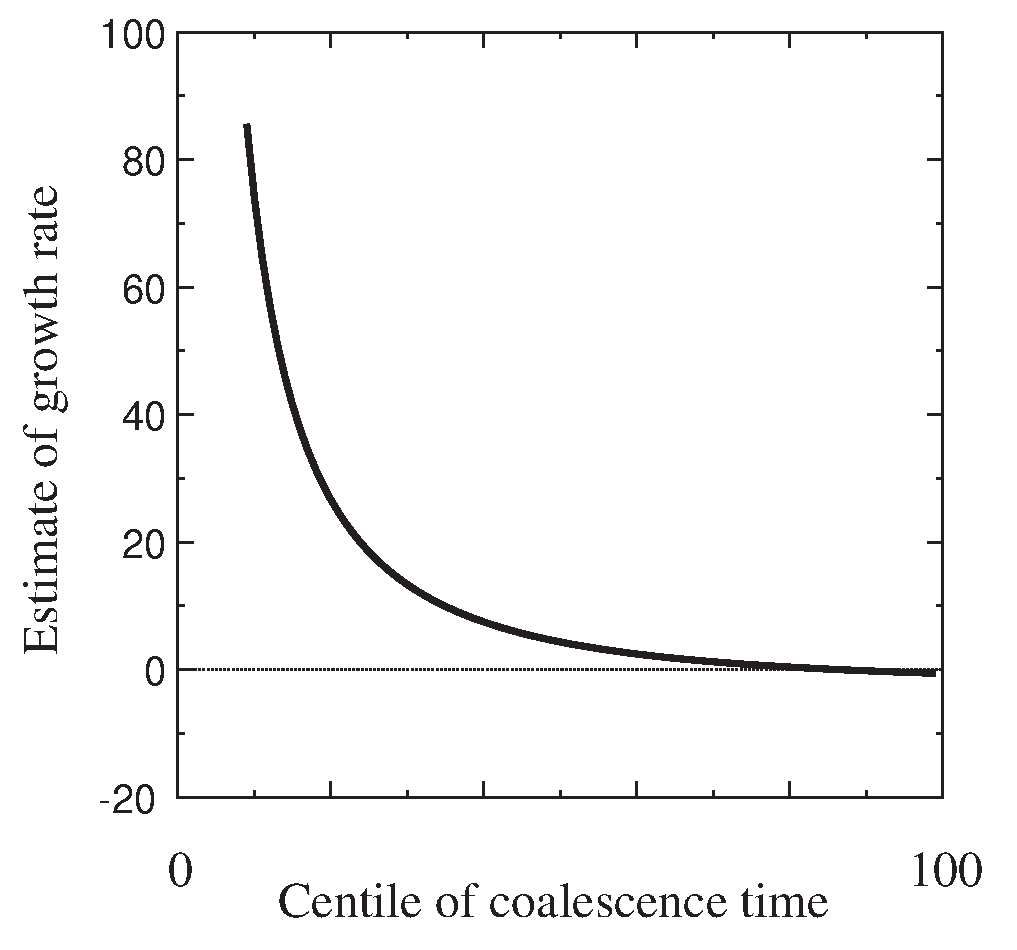
\includegraphics[width=4.5in]{fig5.ps}}
\caption{Estimates of growth rate for $n=2$ in a data set with a large number of sites,
so that coalescence time can be estimated accurately.  For a case where
$\Theta$ is known and the true growth rate is 0, the estimates for
different quantiles of the coalescence time are shown.  A large bias toward
inferring growth is apparent.}
\end{figure}

This bias sounds like a serious problem for Monte Carlo integration
methods.  It is, but we are convinced that it is an equally serious
problem for all other methods.  However, although the point estimates
are biased, if we make interval estimates using the usual chi-square
approximation to the distribution of the likelihood ratio, accepting
all values of $g$ whose log-likelihood is within 3 units of the peak
(in the more general case where two parameters, $g$ and $\Theta$, are being
estimated), the true value
of 0 is within the interval almost 95\% of the time.  
In this case (S. Tavar\'e, pers. comm.) the chi-square distribution is of
dubious propriety, as it has an asymptotic justification but is being used on
data from a single locus.  Nevertheless, the interval based on it seems to
behave appropriately.  In addition,
the bias becomes much smaller as we add data from more loci \cite{Kuhner98}.

\section{Migration.}  We can also extend the model to allow for multiple
populations exchanging migrants.  This has been done by Nath and Griffiths
\cite{Nath96}, who estimate the migration rates for populations whose values of
$\Theta$ are known.  We have \cite{Beerli99} extended our Metropolis-Hastings
method to a two-population case, to estimate the two values of $\Theta$
and two migration rates.  This seems to have advantages over methods
using statistics like $F_{ST}$, as those cannot estimate all four
parameters independently.  An extension to $n$ populations is in progress.

\section{Sequential Sampling.}  In studies of ancient DNA, we have samples
that are not contemporaneous.  In studies of the course of viral infection
in a patient (as in HIV) one may also have sequential samples.  The
coalescent likelihood approach is readily adapted to such cases
\cite{Rodrigo98}.  Suppose
that we have a genealogical tree $G^*$ whose branch lengths are
actual times, with some tips not contemporaneous.    Let the generation
time of the organism be $\tau$.  As one proceeds down the tree, there are
two possible events, the entry of a new sample (which has probability 1
at certain known times) or a coalescence.  In place of equation \ref{eq:basic},
we have a product of terms, the $j$-th of which is either
\begin{equation} % 9.1
\frac{2}{4N_e} \exp\left[-{k_j(k_j-1) \over 4N_e } {u_j \over \tau} \right]
\end{equation}
or
\begin{equation} % 9.1
\exp\left[-{k_j(k_j-1) \over 4N_e } {u_j \over \tau} \right]
\end{equation}
depending on whether there is a coalescence or a new sample at the bottom
end of interval $j$.  Note that $k_j$ is the number of lineages that exist
in the genealogy during interval $j$.  Note also that the chronological
lengths of the interval have been divided by the generation time to convert
them into generation times.  The probability of the data given $G^*$ also
needs a
conversion: it depends on the product of the per-generation mutation rate per
site, $\mu$ and the generation time elapsed, which is $t/\tau$.

The result is that we can restate equation \ref{eq:intG} as 
\begin{equation} % 9.2
\Prob\left(D|N_e\tau, \mu/\tau\right) = \int_{G^*} f(G^*|N_e\tau) \Prob(D|G^*, \mu/\tau).
\end{equation}
so that the two parameters that can be estimated are $N_e\tau$ and $\mu/\tau$.
This means that if we know the generation time $\tau$ we can estimate
$N_e$ and $\mu$ separately.  Alternatively if (for example) we know $\mu$,
we can estimate $N_e$ as well as the generation time $\tau$.  Note that the
integration over $G^*$ would involve all possible labelled histories and
coalescent times, but would not alter the times at which the samples were
taken, these being assumed known.

\section{Recombination.}  All of the above cases involve sequences with
no recombination.  They are thus appropriate for mitochondrial DNA but
of dubious value in the nuclear genome.  For this reason it has been of
great interest to everyone involved with coalescent likelihood methods to
have a way of dealing with recombination.  As usual, we have come in
second in the race, as Griffiths and Marjoram \cite{GM96} have an
algorithm
that infers the likelihood of a sample with two parameters, $4N_e\mu$
and $4N_ec$, where $c$ is the recombination fraction per site.  Their
method requires substantial computation to adequately sample the histories.
Their method makes use of an ``ancestral recombination graph" \cite{GM97}
originally described by Hudson \cite{Hudson90}.  This shows coalescences and recombination
events.  The latter branch as one goes rootwards, and at each such branching
one needs to specify which sites take each of the two routes.

We have also produced a program for inferring these two parameters,
[manuscript in preparation].  Although the Metropolis-Hastings approach
helps concentrate the sampling on the relevant genealogies, the number of
these is so large that the computation is still slow.  Figure 6 shows contours
of a likelihood surface produced in one of our runs.
\begin{figure} % 6
\centerline{\includegraphics[width=4.5in]{fig6.ps}}
\caption{Contours of the likelihood surface from a single run of a
the {\tt RECOMBINE} Metropolis-Hastings sampler with recombination on simulated data.  The axes are $\Theta=4N_e\mu$
and the recombination parameter $c/\mu$.  The contours shown are
$1, 2, 3, \ldots$ units of log-likelihood below the peak. The true values of
the parameters are shown by the dashed lines. In this run the value of $\Theta$
is a bit higher than the truth, but the true parameters lie well within the
contour of 3 log-likelihood units below the peak, which defines their approximate }
confidence limits.
\end{figure}
There are serious problems ahead, as we need to know how long to run the
Markov chains to get an accurate answer, and this is generally unknown.
However there are also opportunities.  One involves using these methods to
place a firm likelihood foundation under the widely used genetic mapping
method known as linkage disequilibrium mapping.  A start has been made on this
by Rannala and Slatkin \cite{Rannala}
and Graham and Thompson \cite{Jinko};
our methods can be used to treat the problem more generally.


\section{Natural Selection.}

Until recently it was assumed by everyone that one could not specify
the coalescent for sequences that were under natural selection.  Only
some special cases could be solved, for cases of extreme selection
\cite{Kaplan88, Hudson88, Takahata90}. Recently Neuhauser and Krone \cite{Neuhauser97, Krone97} made major inroads into the
problem, in what are perhaps the best papers on the coalescent since
Kingman.  They defined a diagram that branches both downward and upward.
Unlike the similar diagrams that are produced in cases of recombination,
these do not have different alleles following different loops.  Instead
information flowing upward on the genealogical graph can only pass through
certain branches if the genotype contains one of the selected alleles.
In the case of recombination, at each site the graph is a tree, although not
the same tree at all sites.  In the Neuhauser-Krone ``ancestral selection
graph" the loops are rather more serious.  If one tries to compute
$\Prob(D|G)$ on them, likelihood must be propagated simultaneously, not
independently, around both sides of a loop.  However, they were able to
define a recursion system that could be evaluated by Griffiths and Tavar\'e's
method.

Neuhauser and Krone's work is an enormous and stimulating advance.  But it
seems ill adapted to our Metropolis-Hastings approach, since 
when the selection coefficient favoring haploid genotype $A_1$ over
genotype $A_2$ is $s$, for moderate
values of $2N_es$ the number of loops in the ancestral selection graph can
become large.  Stimulated by it, J.F. has started work on a different method,
which involves carrying out Metropolis-Hastings simulation of the
frequencies of the selected alleles, as well as the coalescent of other
alleles within those alleles, and the ``migration" between them that is caused
by mutation and recombination.  There are no results to report yet.

\section{Software Distribution}

Our package {\tt LAMARC} (which stands for Likelihood Analysis by
Metropolis Algorithm for Random Coalescents) is available free from its
Web site:\\
{\tt \ \ \ \ \ http://evolution.genetics.washington.edu/lamarc.html}\\
as C source code plus PowerMac and Windows executables.  It is readily
compiled on workstation C compilers (except for the {\tt cc}
compiler on SunOS systems).  As of this writing four programs were
in distribution: {\tt COALESCE}, which analyzes a single population of
constant size, {\tt FLUCTUATE}, which analyzes exponentially growing
single populations, {\tt MIGRATE}, which analyzes two populations
exchanging migrants, and {\tt RECOMBINE}, which analyzes a single
population of constant size with recombination.  More programs and more features will probably
be available by the time you read this.

\section{An Object-Oriented Fantasy.}

Even if we could solve some of the problems of how long to run the Markov
Chains, the sampling approach has one other serious problem.  We like to
call it ``the $2^8$ programs problem".  Each one of these Markov Chain Monte
Carlo programs is enormously difficult to write.  It takes each of us about
2 years to write and debug one of them.  And yet, the present programs are
highly limited.  We have programs that add one complication (population
growth, migration, recombination) but do not combine these in the same
program.  And yet there are more complications (such as natural selection,
speciation, and gene conversion) that need to be considered.  Any user may
want to pick some particular combination of, say, 8 complications.  Do we
need to resign ourselves to spending the next 500 years writing all possible
programs?  

There is one way out.  Object-oriented programming methods (such as are
embodied in C++, Objective C and Java) allow a program to self-assemble in
response to a user's requirements.  We therefore intend to try to create
such an environment.  The user would select which combination of evolutionary
forces, historical events, genetic situations, and population structure
were needed.  The program would then use only those classes and subclasses
needed to run that particular combination.  Thus more like 8 programs than
$2^8$ need to be written.  The issue of chain length remains, and we as
yet have no experience with the serious issue of user interface -- how do we
represent the results of runs that have many parameters, for example?

Nevertheless one may fantasize about an ``evolutionary genetics black box".
The user puts in the data and the model, and out come likelihood inferences
about the parameters.  One still needs to know population genetic theory,
of course, to comprehend the model.  But a large fraction of the kind of
work that has filled theoretical journals in population genetics may become
obsolete if this fantasy can be realized.  Many papers start with a theoretical
model, pose the question of what is the expected value of some statistic
(such as the probability of monomorphism, or of fixed differences between
populations,
or the variance of heterozygosity), and after much blood, sweat, and tears
arrive at a power series, which usually remains unused by those with data.
We may hope that this era can be succeeded by one where the same effort can be
redirected to formulating the model and improving the computational methods.

\section*{Acknowledgments.} 

We wish to thank Dick Hudson, Robert Griffiths, Simon Tavar\'e, and Kermit
Ritland for helpful communications.

%INSERT ANY THANKS HERE

\begin{thebibliography}{20}
\footnotesize

%INSERT REFERENCE LIST HERE

\bibitem{Kingman82a}
Kingman, J. F. C. 1982.  The coalescent.  {\it Stochastic Processes and Their
Applications}  {\bf 13}: 235-248.

\bibitem{Kingman82b}
Kingman, J. F. C. 1982.  On the genealogy of large populations.  {\it
Journal of Applied Probability}  19A: 27-43.

\bibitem{Kingman82c}
Kingman, J. F. C. 1982.  Exchangeability and the evolution of large populations.
pp. 97-112 in Koch, G. and F. Spizzichino, eds. {\it Exchangeability in
Probability and Statistics. Proceedings of the International Conference on
Exchangeability in Probability and Statistics, Rome, 6th-9th April, 1981, in
honour of Professor Bruno de Finetti}. North-Holland Elsevier, Amsterdam.

\bibitem{Kimura68}
Kimura, M.  1968.  Evolutionary rate at the molecular level.  
{\it Nature} 217: 624-626

\bibitem{Kimura83}
Kimura, M. 1983.  {\it The Neutral Theory of Molecular Evolution.}
Cambridge: Cambridge University Press.

\bibitem{Fels81}
Felsenstein, J.  1981.  Evolutionary trees from DNA sequences: a maximum
likelihood approach.  {\it Journal of Molecular Evolution} 17: 368-376.

\bibitem{Yang93}
Yang, Z.  1993.  Maximum-likelihood estimation of phylogeny from DNA sequences
when substitution rates differ over sites.  {\it Molecular Biology and
Evolution}  10: 1396-1401.

\bibitem{Yang94}
Yang, Z.  1994.  Maximum likelihood phylogenetic estimation from DNA sequences
with variable rates over sites: approximate methods.  {\it Journal of Molecular
Evolution}  39: 306-314.

\bibitem{Yang95}
Yang, Z.  1995.  A space-time process model for the evolution of DNA sequences.
{\it Genetics}  139: 993-1005.

\bibitem{Fels96}
Felsenstein, J. and G. A. Churchill. 1996.
A Hidden Markov Model approach to variation among sites in rate of evolution
{\it Molecular Biology and Evolution}  13: 93-104.

\bibitem{Fels88}
Felsenstein, J. 1988. Phylogenies from molecular sequences: inference and
reliability.  {\it Annual Review of Genetics} 22: 521-565.

\bibitem{Fels92}
Felsenstein, J.  1992.  Estimating effective population size from
samples of sequences: inefficiency of pairwise and segregating sites
as compared to phylogenetic estimates.  {\it Genetical Research}  59: 139-147.

\bibitem{Edwards70}
Edwards, A. W. F.  1970.  Estimation of the branch points of a branching
diffusion process. {\it Journal of the Royal Statistical Society B} 32: 155-174.

\bibitem{Metropolis53}
Metropolis, N., A. W. Rosenbluth, M. N. Rosenbluth, A. H. Teller, and E.
Teller. 1953.  Equation of state calculations by fast computing machines.
{\it Journal of Chemical Physics}  21: 1087-1092.

\bibitem{Hastings70}
Hastings, W. K.  1970.  Monte Carlo sampling methods using Markov chains
and their applications.  {\it Biometrika} 57: 97-109.

\bibitem{Kuhner95}
Kuhner, M. K., J. Yamato, and J. Felsenstein. 1995.
Estimating effective population size and mutation rate from sequence data
using Metropolis-Hastings sampling. {\it Genetics}  140: 1421-1430.

\bibitem{Kuhner97}
Kuhner, M. K., J. Yamato, and J. Felsenstein  1997.  Applications of
Metropolis-Hastings genealogy sampling.  pp. 183-192 in {\it Progress in Population
Genetics and Human Evolution}, ed. P. Donnelly and S. Tavare.  IMA Volumes in
Mathematics and its Applications, volume 87.  Springer Verlag, Berlin.

\bibitem{Shuying}
Li, S., D. K. Pearl, and H. Doss.  1998.
Phylogenetic tree construction using Markov chain Monte Carlo.  Technical
Report No. 583, Department of Statistics, Ohio State University, Columbus,
Ohio.

\bibitem{Ward91}
Ward, R. H.,  B. L. Frazier,  K. Dew-Jager, and S. Paabo.  1991.
Extensive mitochondrial diversity within a single Amerindian tribe.
{\it Proceedings of the National Academy of Sciences, USA} 88: 8720-8724

\bibitem{GT94a}
Griffiths, R. C. and S. Tavar\'e.  1994.
Sampling theory for neutral alleles in a varying environment.
{\it Philosophical Transactions of the Royal Socety of London, Series B (Biological Sciences)} 344: 403-10.

\bibitem{GT94b}
Griffiths, R. C. and S. Tavar\'e.  1994.  Ancestral inference in population
genetics.  {\it Statistical Science}  9: 307-319.

\bibitem{GT94c}
Griffiths, R. C. and S. Tavar\'e  1994.  Simulating probability distributions in the coalescent.
{\it Theoretical Population Biology}  46: 131-159.

\bibitem{Griffiths89}
Griffiths, R. C.  1989.  Genealogical tree probabilities in the
infinitely-many-site model.  {\it Journal of Mathematical Biology} 27:
667-680.

\bibitem{Kuhner98}
Kuhner, M. K., J. Yamato, and J. Felsenstein.  1998.  Maximum likelihood
estimation of population growth rates based on the coalescent. {\it Genetics,}
in press.

\bibitem{Nath96}
Nath, H. B. and R. C. Griffiths.  1996.  Estimation in an island model using
simulation.  {\it Theoretical Population Biology}  50: 227-253.

\bibitem{Beerli99} Beerli, P. and J. Felsenstein. 1999.  Maximum likelihood
estimation of migration rates and effective population numbers in two
populations using a coalescent approach.  {\it Genetics}, in press.

\bibitem{Rodrigo98}
Rodrigo, A. G. and J. Felsenstein. 1998.  Coalescent approaches
to HIV-1 population genetics. in press in {\it Molecular Evolution of HIV,} ed.
K. A. Crandall.  Johns Hopkins University Press, Baltimore.

\bibitem{GM96}
Griffiths, R. C. and P. Marjoram.  1996.  Ancestral inference from samples of
DNA sequences with recombination.  {\it Journal of Computational Biology}
3: 479-502.

\bibitem{GM97}
Griffiths, R. C. and P. Marjoram.  1997. An ancestral recombination graph.
pp. 257-270 in {\it Progress in Population Genetics and
Human Evolution,} ed. P. Donnelly and S. Tavar\'e.  IMA Volumes on
Mathematics and Its Applications, volume 87.  Springer, New York.

\bibitem{Hudson90}
Hudson, R. R.  1990.  Gene genealogies and the coalescent process.
{\it Oxford Surveys in Evolutionary Biology}  7: 1-44.

\bibitem{Rannala}
Rannala, B. and M. Slatkin.  1998.
Likelihood analysis of disequilibrium mapping, and related
problems.  {\it American Journal of Human Genetics} 62: 459-473.

\bibitem{Jinko}
Graham, J. and E. A. Thompson. 1998.  Disequilibrium likelihoods for fine-scale
mapping of a rare allele.  {\it American Journal of Human Genetics} 63: 1517-1530.

\bibitem{Kaplan88}
Kaplan, N. L., T. Darden, and R. R. Hudson.  1988.  The coalescent process
in models with selection.  {\it Genetics}  120:  819-829.

\bibitem{Hudson88}
Hudson, R. R. and N. L. Kaplan.  1988.  The coalescent process in models
with selection and recombination.  {\it Genetics}  120: 831-840.

\bibitem{Takahata90}
Takahata, N.  1990.  A simple genealogical structure of strongly balanced
allelic lines and trans-species evolution of polymorphism.
{\it Proceedings of the National Academy of Sciences, USA}  87: 2419-2423.

\bibitem{Neuhauser97}
Neuhauser, C., and S. M. Krone. 1997.  The genealogy of samples in models
with selection.  {\it Genetics} 145: 519-534.

\bibitem{Krone97}
Krone, S. M. and C. Neuhauser.  1997.  Ancestral processes with selection.
{\it Theoretical Population Biology} {\bf 51:} 210-237.

\end{thebibliography}

% This sample shows the setting for two addresses (two authors)
\Line{\AOSaddress{Department of Genetics\\
University of Washington\\
Box 357360\\
Seattle, Washington 98195-7360\\
joe@genetics.washington.edu}\hfill
}

\end{document}
